\chapter{Implementace}

Grafické uživatelské rozhraní je implementováno knihovnou System.Windows.Forms. Aplikace by měla fungovat rychle, proto je priorita procesu nastavena na RealTime.

Aplikace musí být odolná proti neplatným vstupům. Veškeré zapisované hodnoty se musí kontrolovat na správný formát a rozsah. Proto není možné zapisovat do jednotlivých komponent pomocí systémové klávesnice, ale pouze klávesnicí aplikace (viz kapitola \ref{ch:dialogy}). Další kontrola je v logické vrstvě aplikace.

V aplikaci jsou dvě hlavní okna, jedno pro výběr pacienta a druhé s detailem vybraného pacienta a jednotlivými kartami. Okna s další funkčností jsou zobrazována jako dialogy.

Po spuštění aplikace se zobrazí okno výběru pacientů s prázdným seznamem pacientů a dialog pro přihlášení. Pro práci s aplikací musí být uživatel přihlášen a mít pracovní poměr na pracovišti, na kterém se tablet nachází.


\section{Přihlášení}

Pro přihlášení slouží jednoduchý dialog s dvěma TextBoxy, pro zadání uživatelského jména a hesla, a dvěma Buttony pro přihlášení a zrušení přihlášení. Uživatelské jméno ve FN Plzeň je vždy uppercase, proto jsou znaky v TextBoxu pro uživatelské jméno také uppercase. Znaky hesla jsou skryty symbolem *. Při úspěšném přihlášení se načtou údaje o uživateli a seznam pacientů na lůžkovém oddělení. Při neúspěšném se zobrazí chybová hláška a údaje z TextBoxů se vymažou.

Přihlašovací dialog je na obrázku \ref{fig:login}.

\begin{figure}[H]
	\centering
	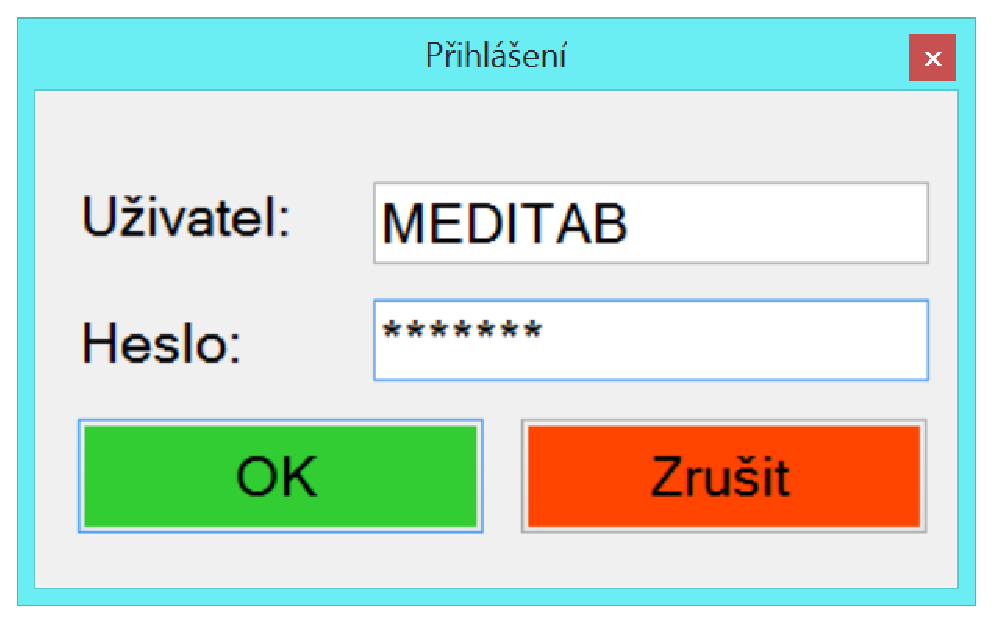
\includegraphics[width=0.5\textwidth]{img/meditab/login.eps}
	\caption{Přihlašovací dialog (MediTab)}
  \label{fig:login}
\end{figure}


\section{Výběr pacienta}

Po úspěšném přihlášení se zobrazí obrazovka se seznamem pacientů (viz obrázek \ref{fig:main}). Seznam pacientů je kolekce v ListView.

V horní části je MenuStrip obsahující dvě položky. První je tlačítko pro odhlášení, které odhlásí aktuálního uživatele a zobrazí dialog pro přihlášení. Druhé tlačítko zobrazí nápovědu k aplikaci. Dole se nachází StatusStrip s informací o přihlášeném uživateli a verzí aplikace. Vravo je Button pro ukončení aplikace.

\begin{figure}[H]
	\centering
	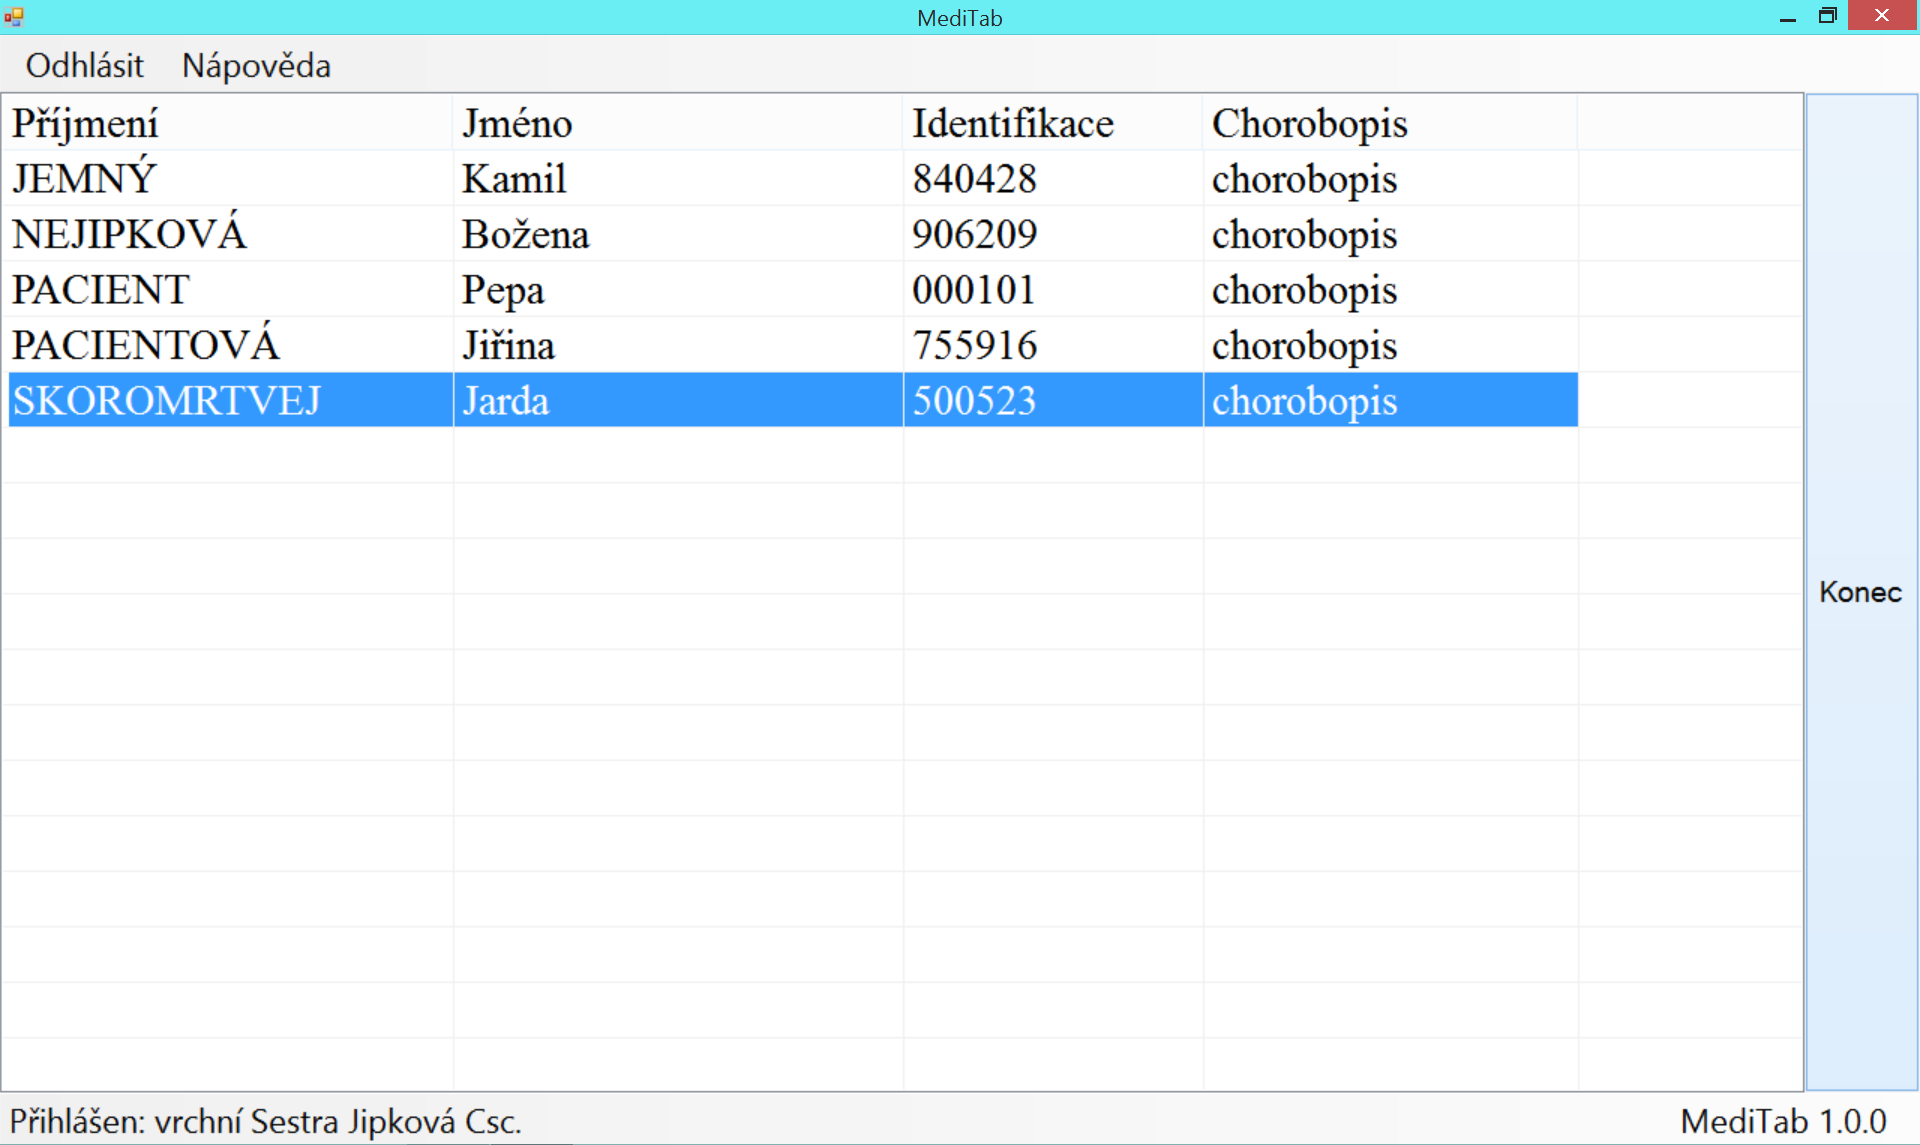
\includegraphics[width=1\textwidth]{img/meditab/main.eps}
	\caption{Výber pacienta (MediTab)}
  \label{fig:main}
\end{figure}


Vybráním pacienta kliknutím na řádek v ListView se začnou stahovat data o pacientovi z databáze, vytvářet a inicializovat jednotlivé záložky. Uživatele o stavu načítání informuje okno viz obrázek \ref{fig:load}.




\section{Detail pacienta}

Hlavní čásní okna detailu pacienta je TabControl pro snadné přepínání mezi jednotlivými záložkami (TabPage). Vpravo je Button pro návrat k výběru pacientů a Button pro zobrazení oprav. Při otevřené záložce denní nebo hodinové bilance tekutin je tam Button pro návrat k výběru pacientů bez uložení hodnot. Vespod je StatusStrip s informací o přihlášeném uživateli, vybraném pacientovi a verzí aplikace.

\subsection{Ordinované léky}

Tabulku ordinovaných léků tvoří dva DataGridView (viz obrázek \ref{fig:medikace}). Oba DataGridView mají synchronizované vertikální scrollování. Scrollováním v jednom se nastaví veritikální offset druhému.

\begin{figure}[H]
	\centering
	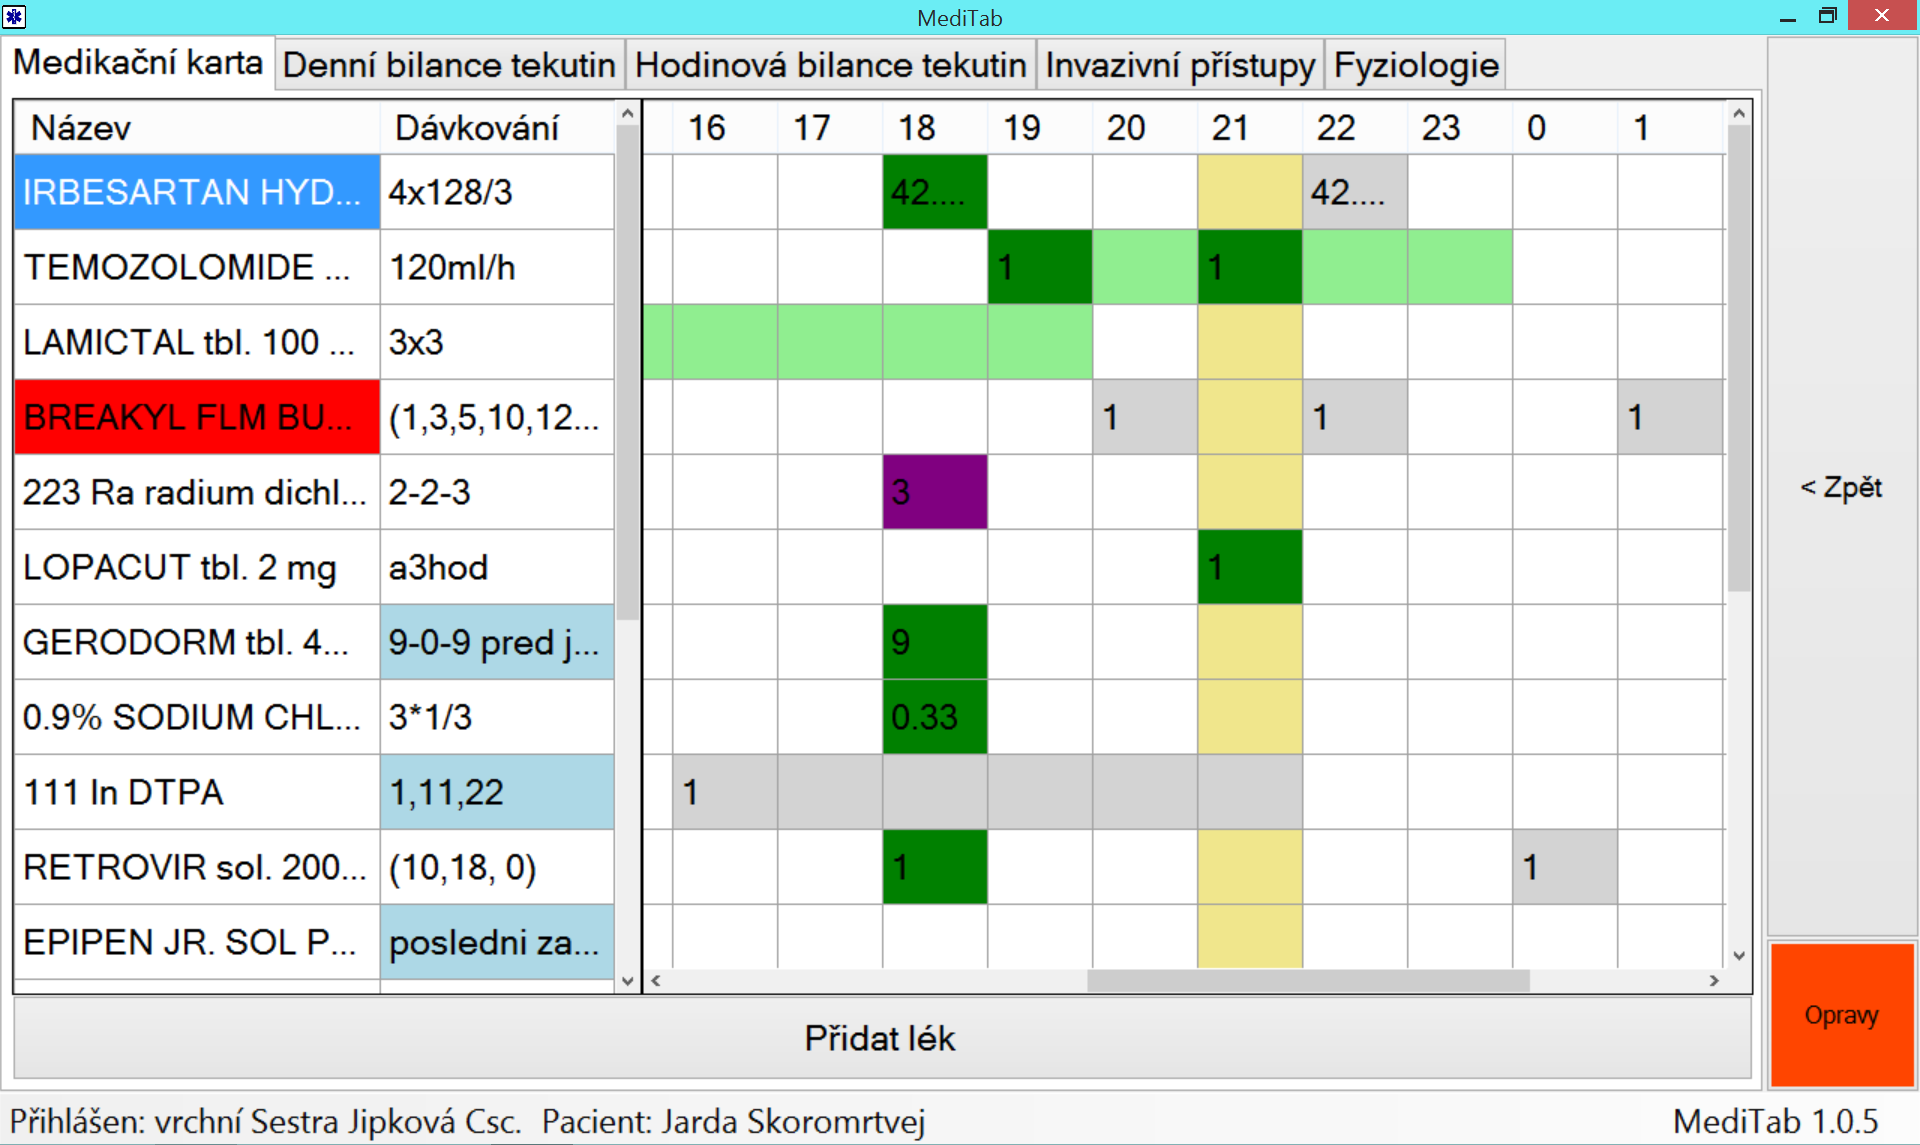
\includegraphics[width=1\textwidth]{img/meditab/medikace.eps}
	\caption{Ordinované léky (MediTab)}
  \label{fig:medikace}
\end{figure}

První DataGridView zobrazuje název léku a dávkování. Pokud je lék opiát, je políčko názvu léku podbarvebo červeně a pokud je u dávkování poznámka, políčko dávkování je podbarveno světle modře.

Druhý DataGridView zobrazuje tabulku jednotlivých ordinací. 24 sloupců představující jednotlivé hodiny je seřazeno od hodiny definované v konfiguraci jako počáteční hodina. Sloupec aktuální hodiny je podbarven khaki barvou vyjma řádek s ordinací v dané hodině. Ordinace má číselnou hodnotu dle množství, které má být/bylo podáno a je podbarvena:

\begin{itemize}
	\item Zeleně - provedená ordinace.
	\item Světle zeleně - provedená infuze (krom hodiny, kde infuze začíná, to je tmavě zelené). Infuze může mít definovaný konec, nebo je zobrazena do aktuální hodiny.
	\item Šedě - ordinovaná ordinace.
	\item Fialově - neprovedená ordinace.
\end{itemize}

Kliknutím na políčko DataGridView se zobrazí dialog podání ordinací (viz kapitola \ref{ch:ordinace} Podání ordinací) s vybranou ordinací (pokud existuje k dané hodině). Po zavření dialogu se aktualizuje celý řádek s lékem. Dvojitým kliknutím se rovnou provede podání ordinace v danou hodinu (podání pouze jednorázové ordinace, ne infuze).

Komponentě DataGridView nelze přiřadit událost Click a DoubleClick tak, aby se při dvojitém kliknutí nevyvolala událost jednoduchého kliknutí. Proto se při prvním kliknutí vytvoří vlákno, které na krátký čas pozastaví vykonání události jednoduchého kliknutí (zobrazení dialogu podání ordinací) a čeká se, jestli v této době uživatel klikne podruhé. Pokud ano, provede se jednorázové podání, pokud ne, zobrazí se dialog podání ordinací.

Vespod záložky je Button pro zobrazení dialogu přidání nového léku (viz kapitola \ref{ch:pridat_lek} Přidání nového léku).


\subsubsection{Podání ordinací}
\label{ch:ordinace}

Dialog podání ordinací rozložením kopíruje dialog ve WinMedicalc (viz obrázek \ref{fig:medikace}). Je rozdělen TableLayoutPanelem na šest části, tři řádky a dva sloupce.

\begin{figure}[H]
	\centering
	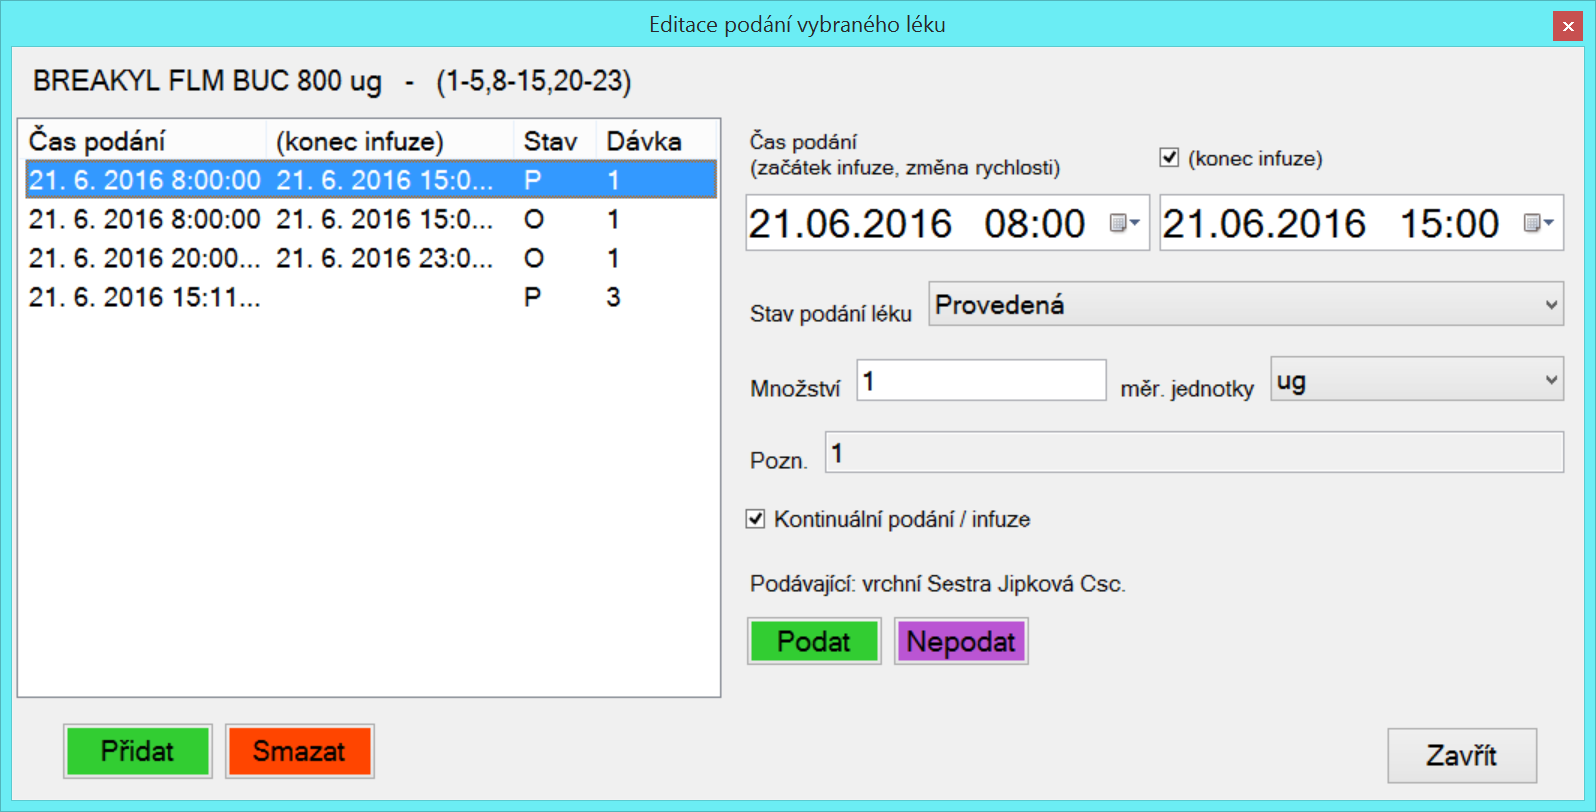
\includegraphics[width=1\textwidth]{img/meditab/ordinace.eps}
	\caption{Podání ordinací (MediTab)}
  \label{fig:ordinace}
\end{figure}

V prvním řádku je název léku a dávkování.

V druhém řádku prvním sloupci je seznam ordinací daného léku v ListView, v druhém sloupci pak detail vybrané ordinace. Vybráním ordinace ze seznamu (FocusedIndex) se zobrazí její detail. Pokud se změní hodnota ordinace, při výběru jiné nebo zavření dialogu se současná uloží a případně se aktualizuje řádek v ListView.

Změna hodin v DateTimePickerech nastane přejetím prstu po komponentě (přímá změna hodnoty není na tabletu vhodná). V okamžiku vstupu do místa DateTimePickeru se uloží y-ová souřadnice, v okamžiku kdy se komponenta opustí se hodina podle místa opuštění zvýší nebo sníží. Pokud ordinace nemá nastaveny vlastní jednotky, zobrazují se jednotky léku. Do poznámky lze zapisovat pouze pokud je stav ordinace nastaven na nepodáno.

V posledním řádku jsou tlačítka na přidání nové ordinace, smazání ordinace a zavření dialogu. Button přidání ordinace vytvoří záznam v ListView ordinací, ale ordinace se uloží až při vybrání jiné ordinace nebo při zavření dialogu. Proto při mazání ordinace se zkontroluje zda je daná ordinace v paměti. Pokud ano, odešle se požadavek na smazání, pokud ne, odstraní se pouze z ListView. Při zavření dialogu proběhne kontrola, zda právě zobrazená ordinace nebyla změněna a případně se uloží.


\subsubsection{Přidání nového léku}
\label{ch:pridat_lek}

Dialog na obrázku \ref{fig:medikace_pridat_lek} umožní sestře přidat nový naordinovaný lék.

\begin{figure}[H]
	\centering
	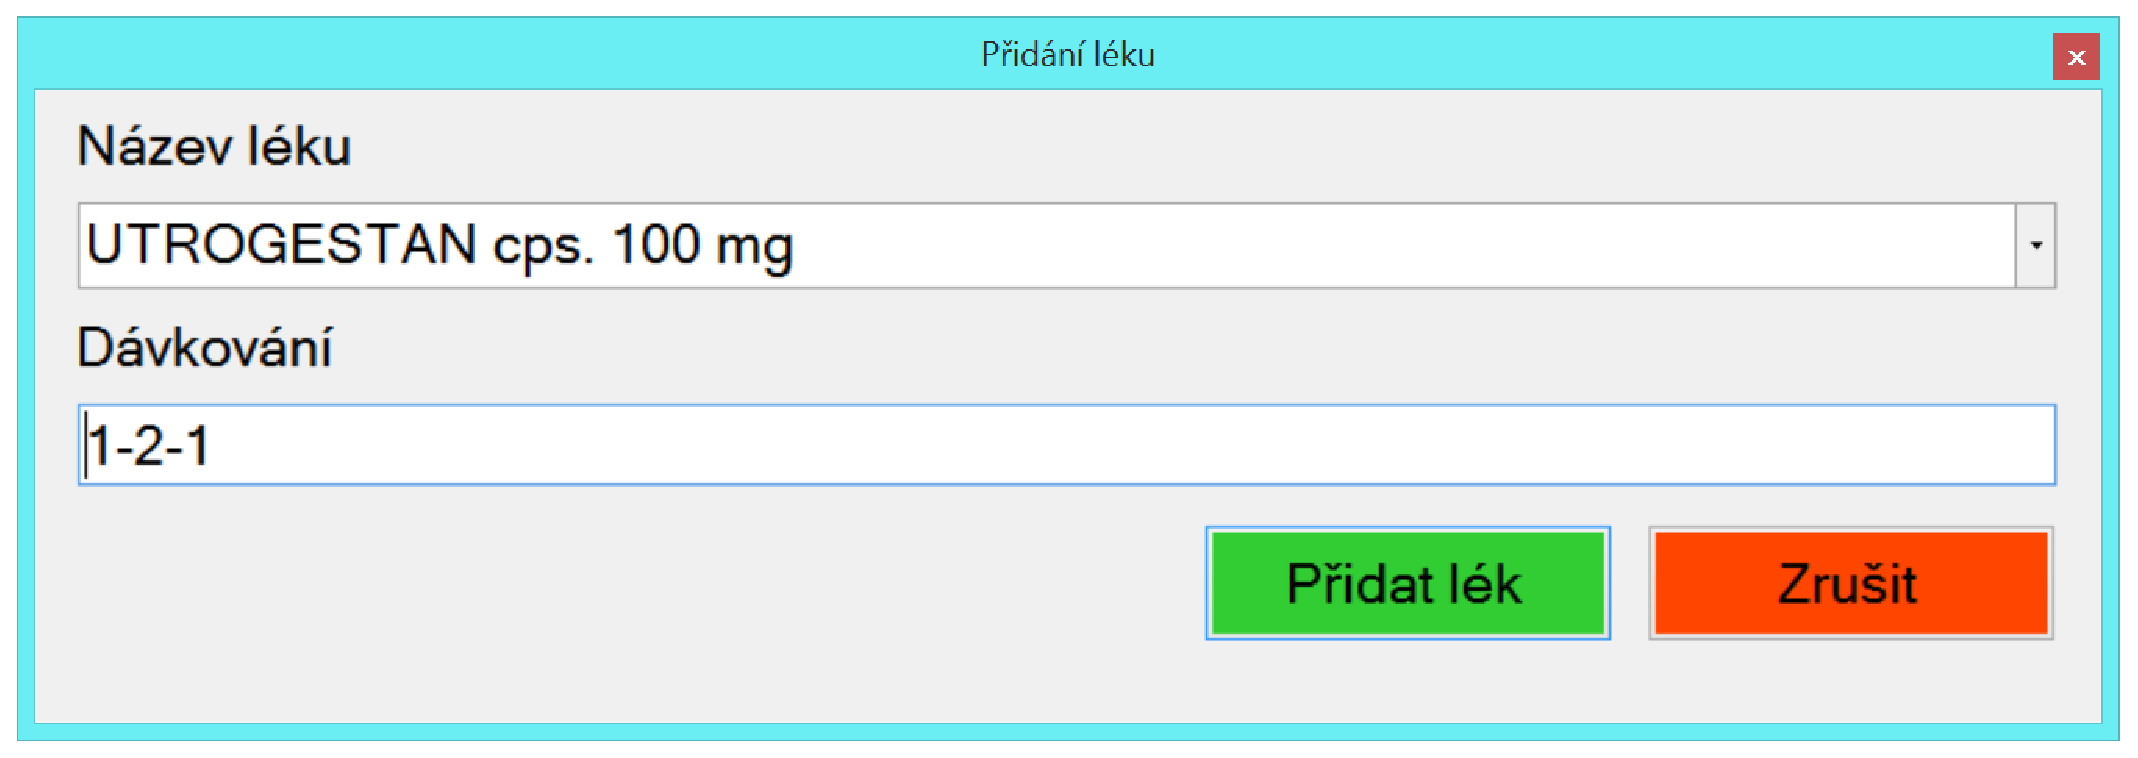
\includegraphics[width=1\textwidth]{img/meditab/medikace_pridat_lek.eps}
	\caption{Přidání nového léku (MediTab)}
  \label{fig:medikace_pridat_lek}
\end{figure}

V ComboBoxu se vybírá lék, který má být naordinován. Jelikož je léků velké množství a většina má více druhů balení, po napsání části názvu léku se v ComboBoxu zobrazí pouze léky obsahující tento text. V dávkování je uživatel k zápisu podle standartů nemocnice, které mohou být rozparsovatelné a následně graficky znázorněné v medikační kartě. Pokud uživatel zadá podání nekorektně nebo vůbec, je o tom informován a předepsání léku s nekorektním dávkováním musí potvrdit.

Po zavření dialogu se nový lék přidá na poslední řádku v medikační kartě.


\subsection{Denní bilance tekutin}

Záložka denní bilance tekutin (na obrázku \ref{fig:bilance_den}) zobrazuje bilanci tekutin za celý den. Je rozdělena SplitContainerem na tekutiny příjmu (zelená) a tekutiny výdeje (červená). Každá tekutina má dva TextBoxy, první zobrazuje celkovou hodnotu za den (lze zadat novou hodnotu větší než původní), v druhém lze přičíst nově naměřenou hodnotu. Poslední hodnotou je celkový součet příjmu a výdeje všech tekutin.

Jednotlivé tekutiny jsou v paměti indexovány podle enumu \emph{Tekutiny}. Stejně tak jsou indexovány TextBoxy celkové hodnoty tekutiny (TabIndex). TextBoxy přičtení nové hodnoty jsou indexovány stejně +100. Při ukládání hodnot se předává index TextBoxu a hodnota.

\begin{figure}[H]
	\centering
	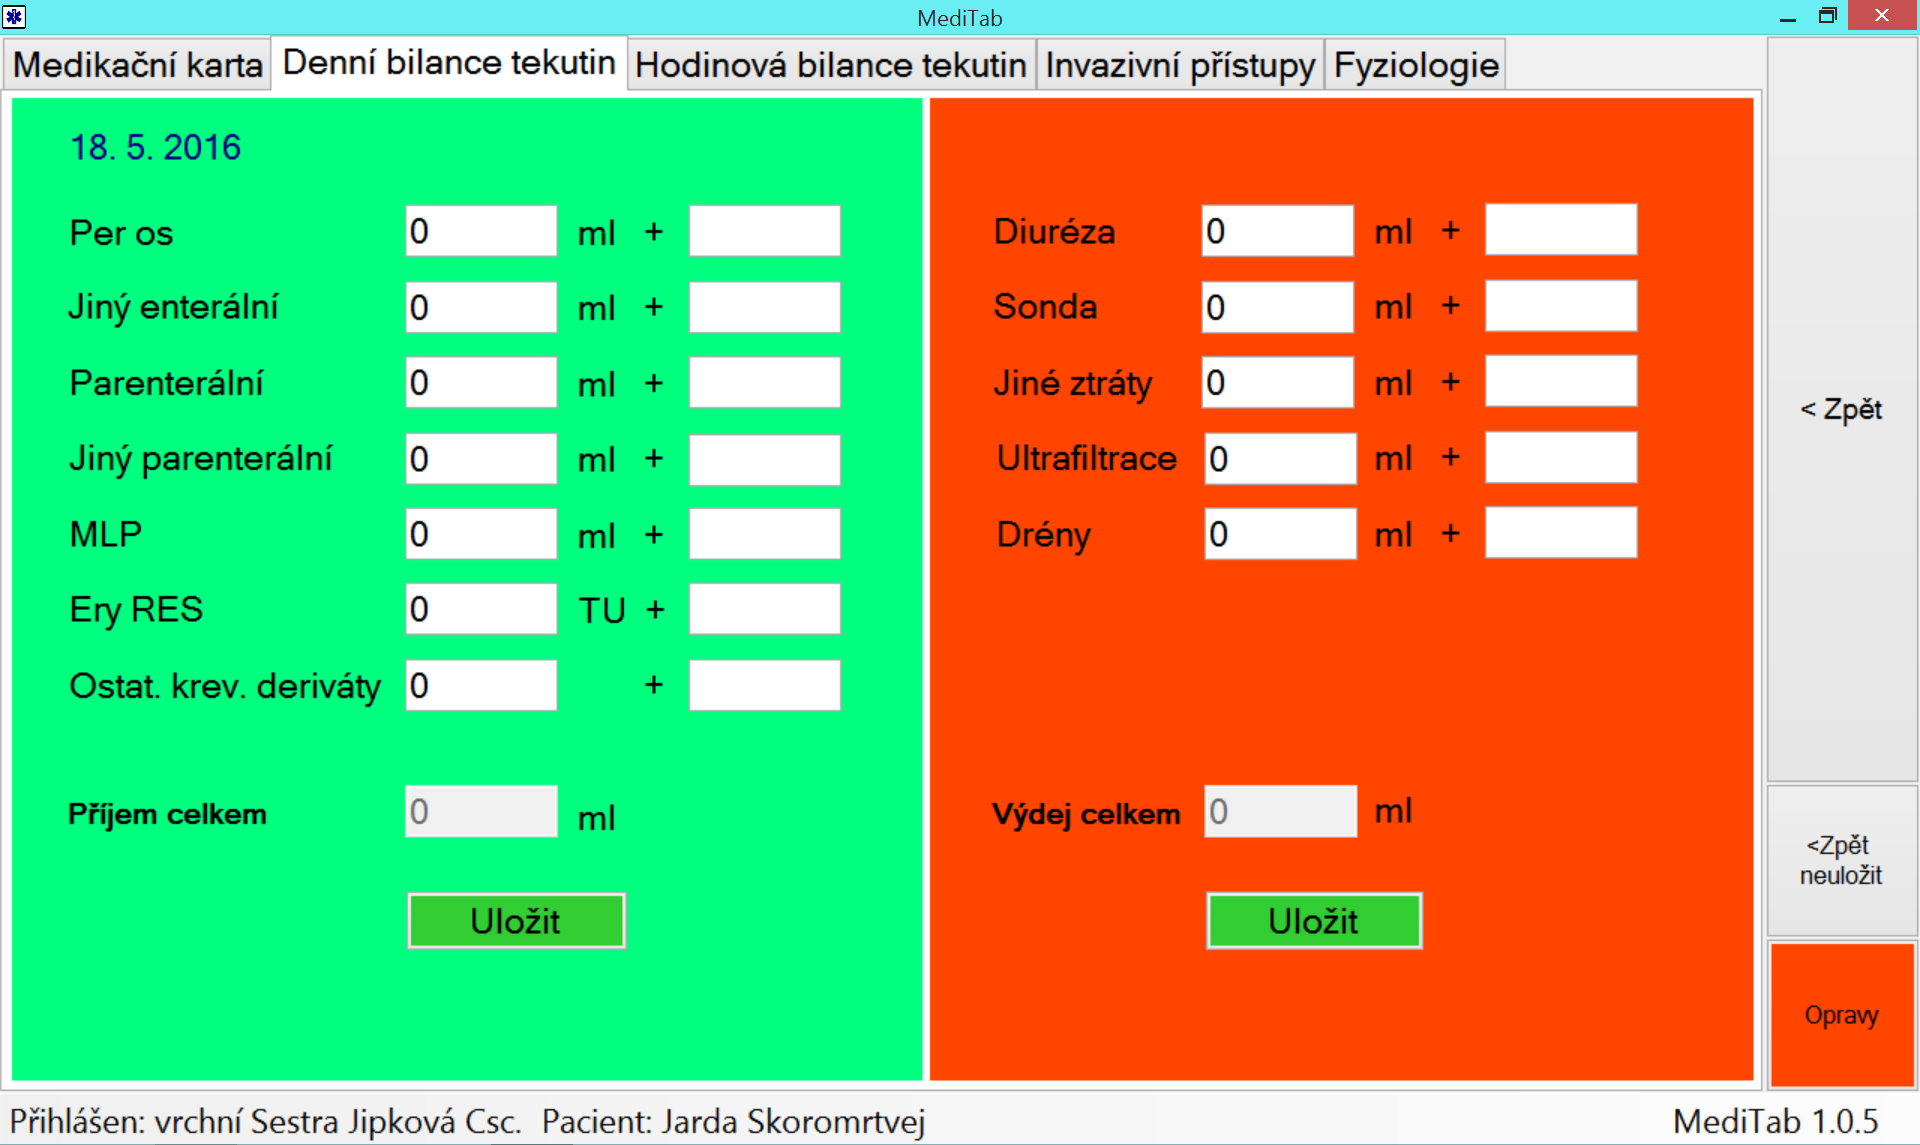
\includegraphics[width=1\textwidth]{img/meditab/bilance_den.eps}
	\caption{Denní bilance tekutin (MediTab)}
  \label{fig:bilance_den}
\end{figure}

Hodnoty se musí uložit kliknutím na Button \emph{Uložit}. Pokud uživatel přepne na jinou záložku aplikace ho upozorní, že hodnoty neuložil a zeptá se, jestli je chce uložit. Buttonem \emph{Zpět} se hodnoty uloží a vrátí se k výběru pacientů, Buttonem \emph{Zpět bez uložení} se vrátí k výběru pacientů bez uložení.

\subsection{Hodinová bilance tekutin}

Záložka hodinové bilance tekutin (na obrázku \ref{fig:bilance_hod}) zobrazuje bilanci tekutin za aktuální hodinu. Je rozdělena SplitContainerem na tekutiny příjmu (zelená) a tekutiny výdeje (červená). Každá tekutina má TextBoxy, který zobrazuje hodnotu v aktuální hodinu (lze zadat pouze jednu hodnotu v hodině) a Button, který zobrazí dialog se všemi hodinami k dané tekutině (viz obrázek \ref{fig:bilance_hod_detail}). Poslední dvě hodnoty jsou celkový součet příjmu a výdeje všech tekutin v dané hodině a za celý den.

Jednotlivé tekutiny jsou v paměti indexovány podle enumu \emph{Tekutiny}. Stejně tak jsou indexovány TextBoxy celkové hodnoty tekutiny (TabIndex). Buttony zobrazení všech hodin jsou indexovány stejně +100 Při ukládání hodnot se předává index TextBoxu hodnota a aktuální hodina.

\begin{figure}[H]
	\centering
	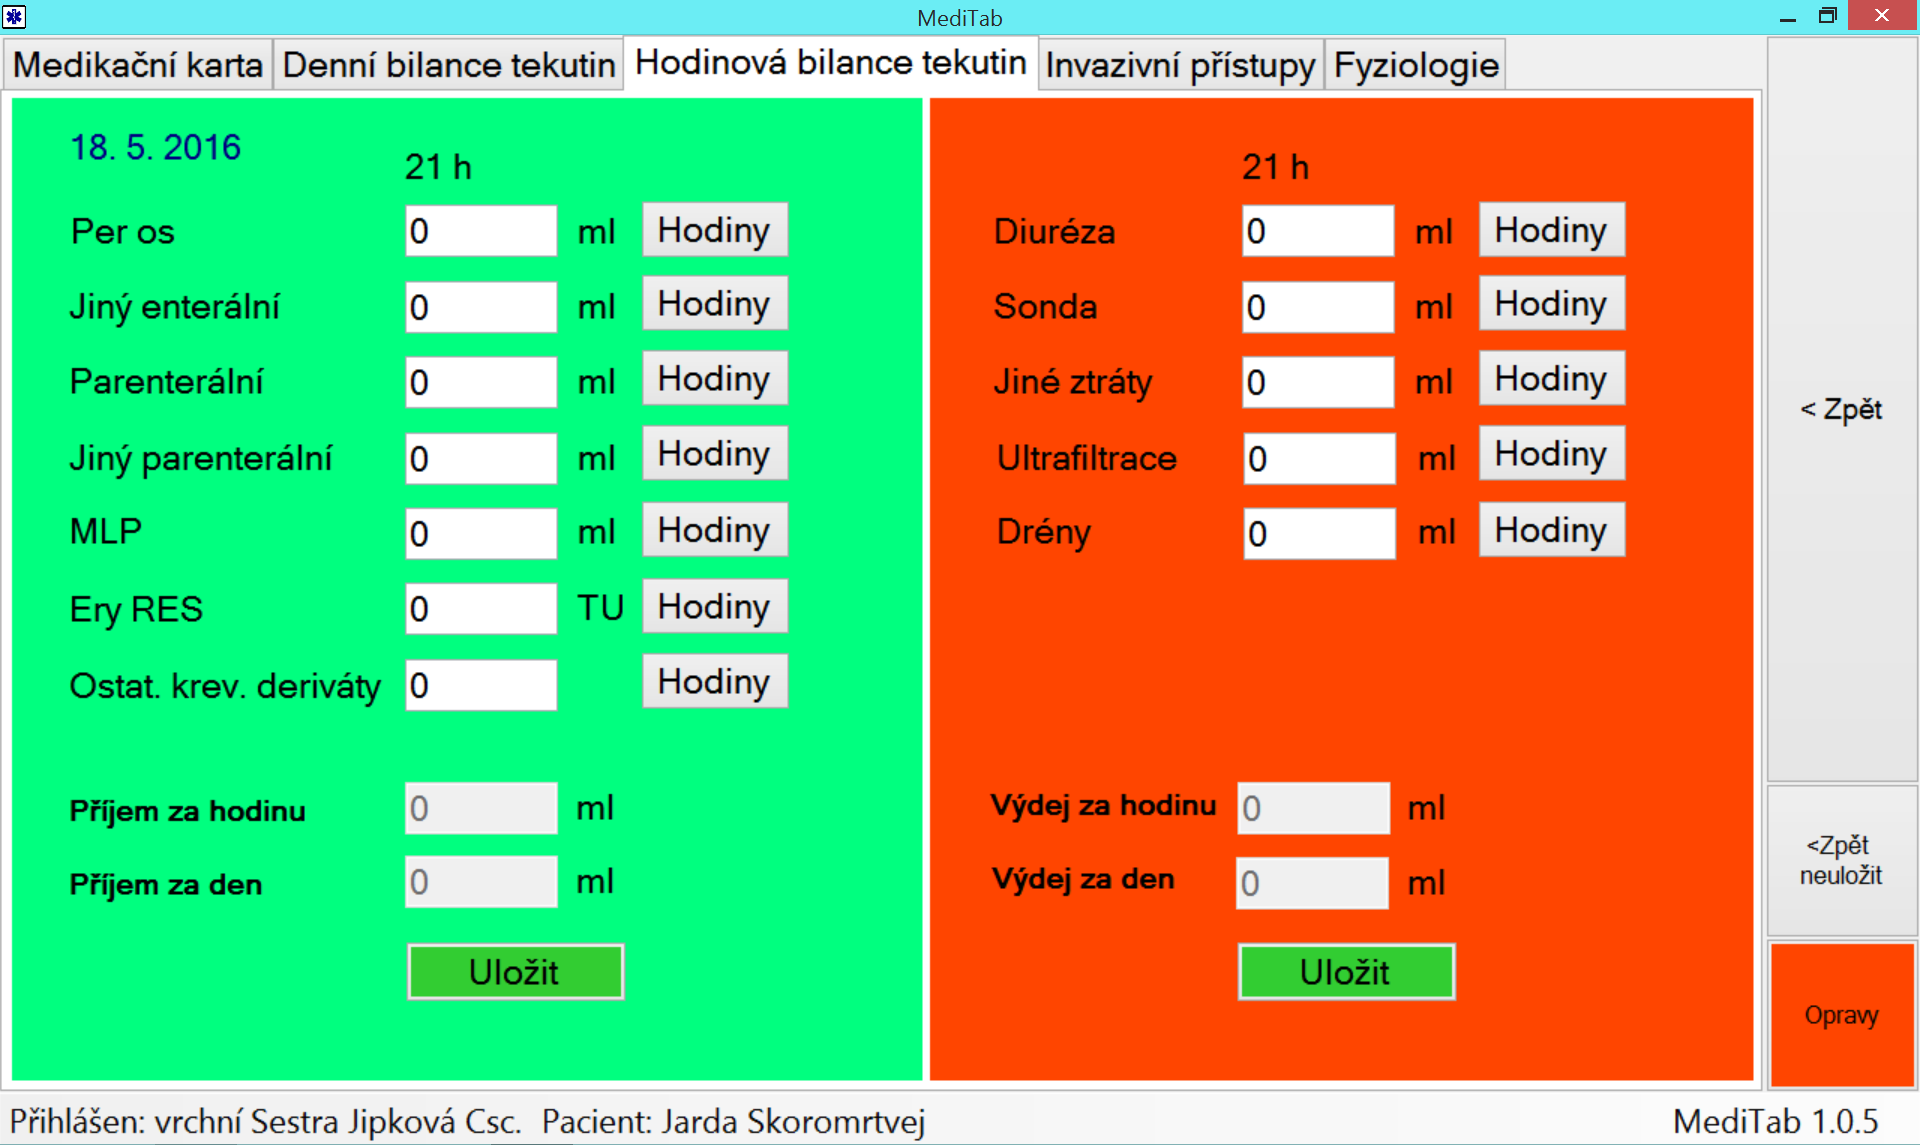
\includegraphics[width=1\textwidth]{img/meditab/bilance_hod.eps}
	\caption{Hodinová bilance tekutin (MediTab)}
  \label{fig:bilance_hod}
\end{figure}

Dialog s hodinovým detailem tekutiny obsahuje DataGridView s dvěma sloupci (hodina, hodnota). Vespod pak je součet všech hodinových hodnot dané tekutiny a tlačítko zavřít. Hodnoty k jednotlivým hodinám lze zadat kliknutím na dané políčko DataGridView. V hodinu lze zadat pouze jednu hodnotu.

\begin{figure}[H]
	\centering
	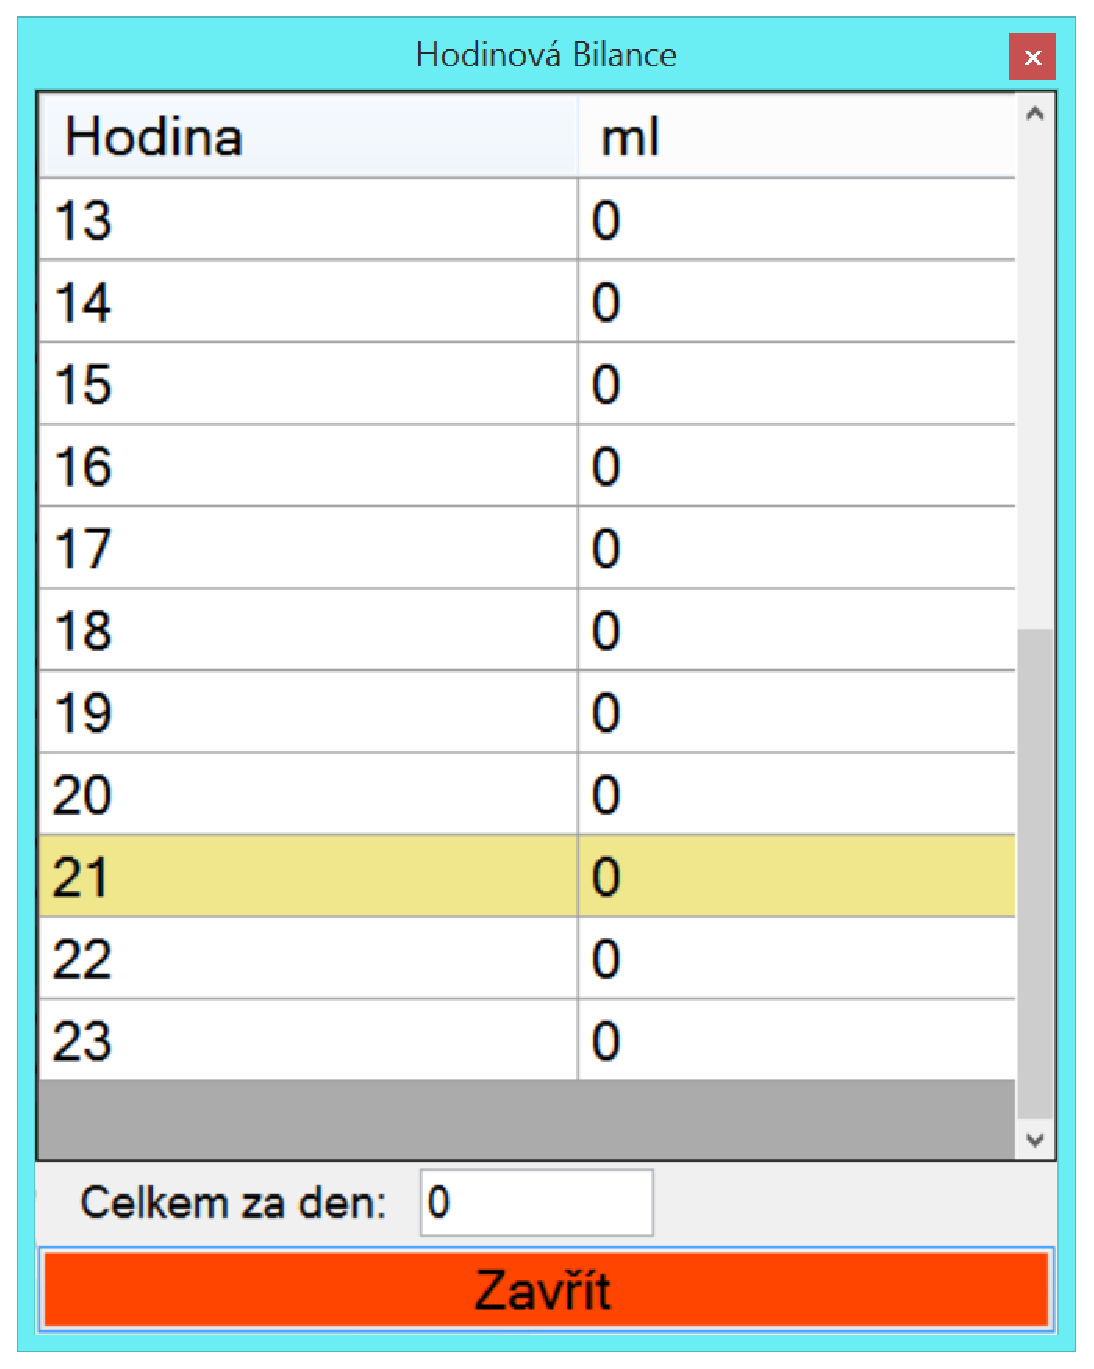
\includegraphics[width=0.3\textwidth]{img/meditab/bilance_hod_detail.eps}
	\caption{Hodinová bilance tekutin - hodinový detail tekutiny (MediTab)}
  \label{fig:bilance_hod_detail}
\end{figure}

Hodnoty se musí uložit kliknutím na Button \emph{Uložit}. Pokud uživatel přepne na jinou záložku, aplikace ho upozorní, že hodnoty neuložil, a zeptá se, jestli je chce uložit. Buttonem \emph{Zpět} se hodnoty uloží a vrátí se k výběru pacientů, Buttonem \emph{Zpět bez uložení} se vrátí k výběru pacientů bez uložení.


\subsection{Invazivní přístupy}
\label{ch:pristup}

V záložce invazivních přístupů (obrázek \ref{fig:invaz_pristup}) je každý invazivní přístup reprezentován vytvořenou komponentou PristupPanel, která dědí od FlowLayoutPanelu. V PristupPanelu jsou veškeré komponenty s informacemi o daném invazivním přístupu (ComboBoxy, TextBoxy, DateTimePicker) a ovládací tlačítka (Vyměnit, Aktualizuj, Vymaž). Panel je na střídačku podbarven ve dvou odstínech světle šedé pro lepší přehlednost.

První panel je pouze s Labely označujícími uspořádání komponent. Poslední panel umožňuje přidání nového invazivního přístupu. Tento panel má místo ovládacích tlačítek Button \emph{Přidat}. Přidáním nového invazivního přístupu se přístup uloží, místo Buttonu \emph{Přidat} zobrazí ovládací tlačítka a do záložky se přidá nový PristupPanel pro přidání dalšího přístupu.

\begin{figure}[H]
	\centering
	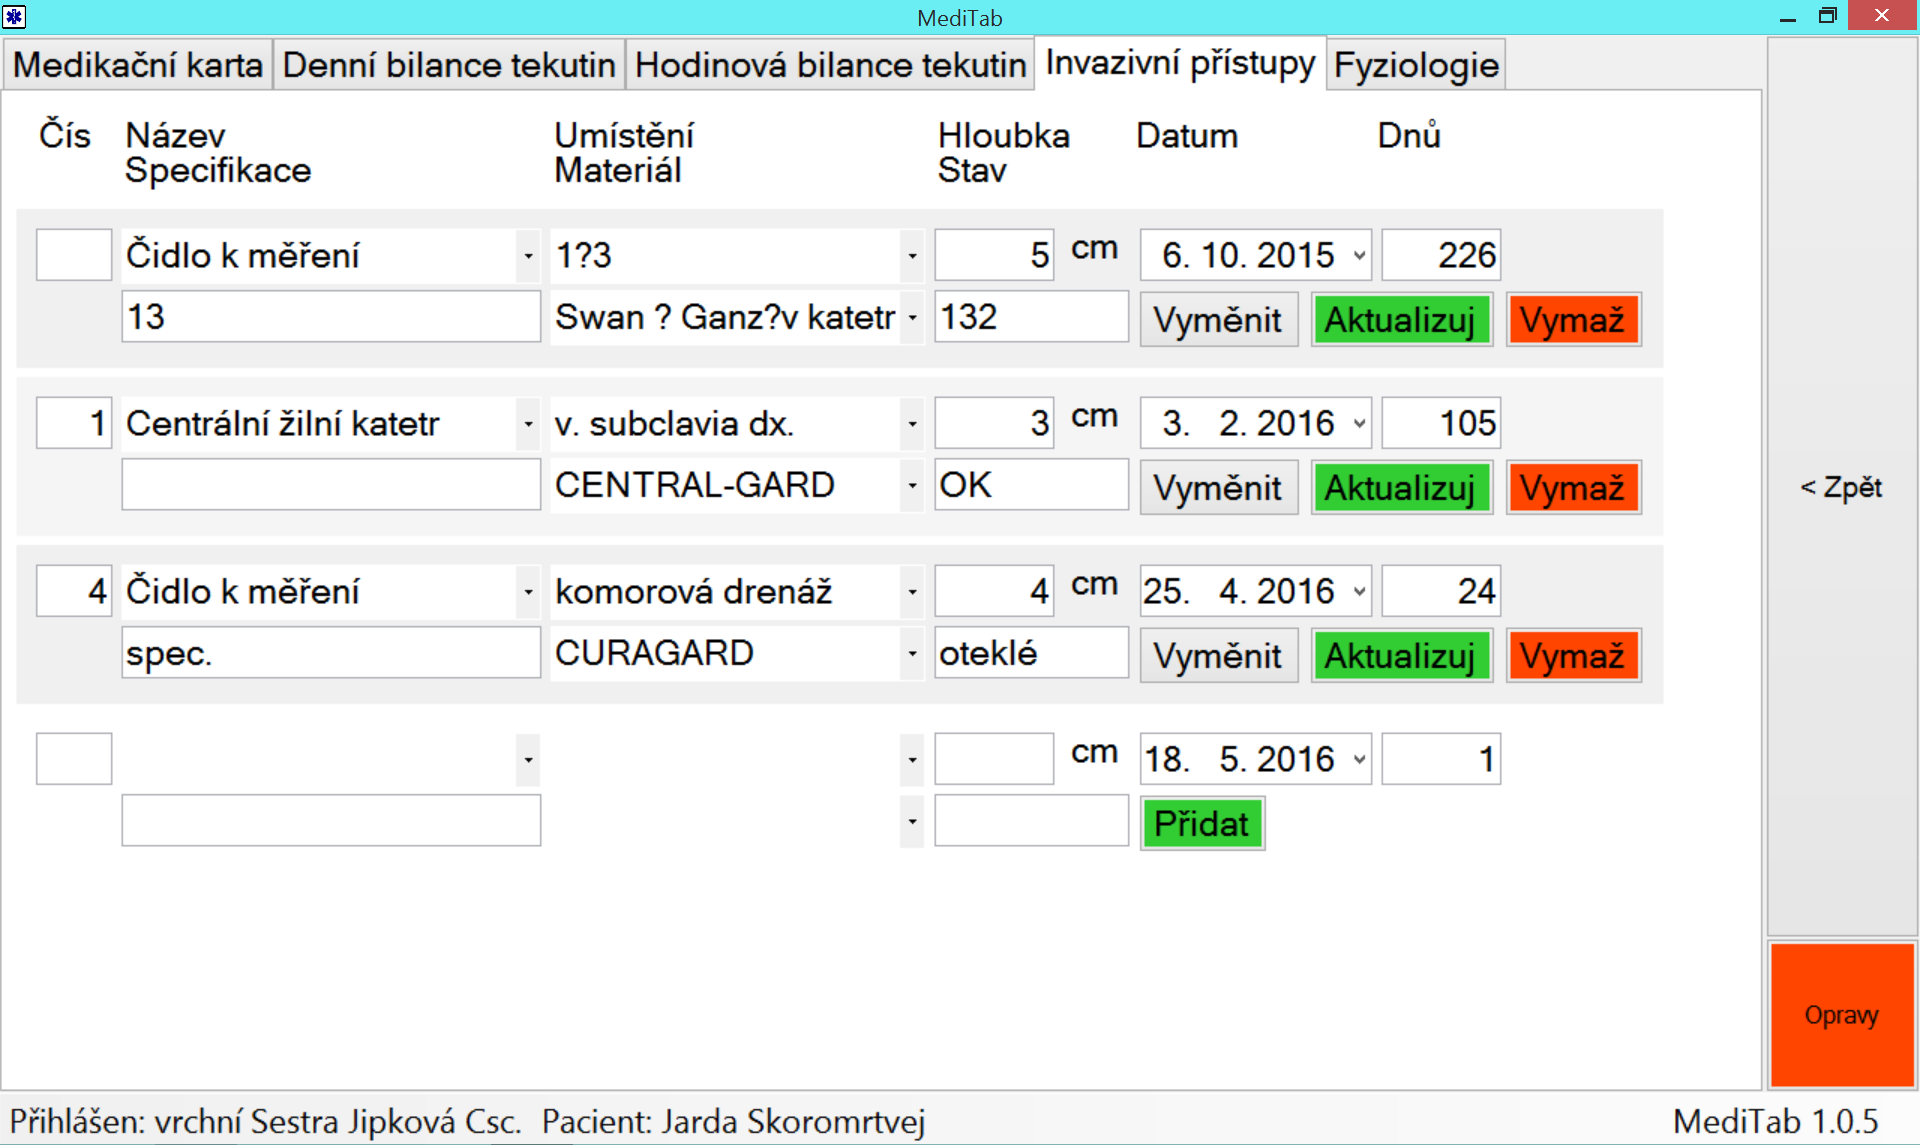
\includegraphics[width=1\textwidth]{img/meditab/invaz_pristup.eps}
	\caption{Invazivní přístupy (MediTab)}
  \label{fig:invaz_pristup}
\end{figure}

Při scrollování tažením prstem na tabletu se vyvolá událost vrchní komponenty, ne kontejneru, ve kterém jsou komponenty umístěny. To jsem vyřešil vytvořením MessageFiltru \emph{MouseFilter} a \emph{TouchableLayoutPanelu}.

MouseFilter monitoruje systémové události, konkrátně stisk levého tlačítka myši (kliknutí prstem), uvolnění levého tlačítka myši a pohyb myši, a odešle je do jejich destinace (tj. komponenta, která se u MouseFilteru zaregistruje jako posluchač). 

TouchableFlowLayoutPanel dědí od FlowLayoutPanelu a má tak stejné vlastnosti. Při jeho vytvoření zaregistruje reakce na scrollování událostem MouseFilteru. Stejně tak se musí zaregistrovat každý PristupPanel.


\subsection{Fyzilologie}

V záložce fyziologie (obrázek \ref{fig:fyziologie}) je každý záznam reprezentován vytvořenou komponentou FyziologiePanel, která dědí od FlowLayoutPanelu. Ve FyziologiePanelu je datum záznamu, TextBoxy s hodnotami životních funkcí pacienta a ovládací tlačítka (Upravit, Smazat).

První panel je pouze s Labely označujícími uspořádání komponent. Poslední panel umožňuje přidání nového záznamu. Tento panel má místo ovládacích tlačítek Button \emph{Přidat}. Přidáním nového záznamu se záznam uloží, místo Buttonu \emph{Přidat} zobrazí ovládací tlačítka a do záložky se přidá nový FyziologiePanel pro přidání dalšího záznamu.

\begin{figure}[H]
	\centering
	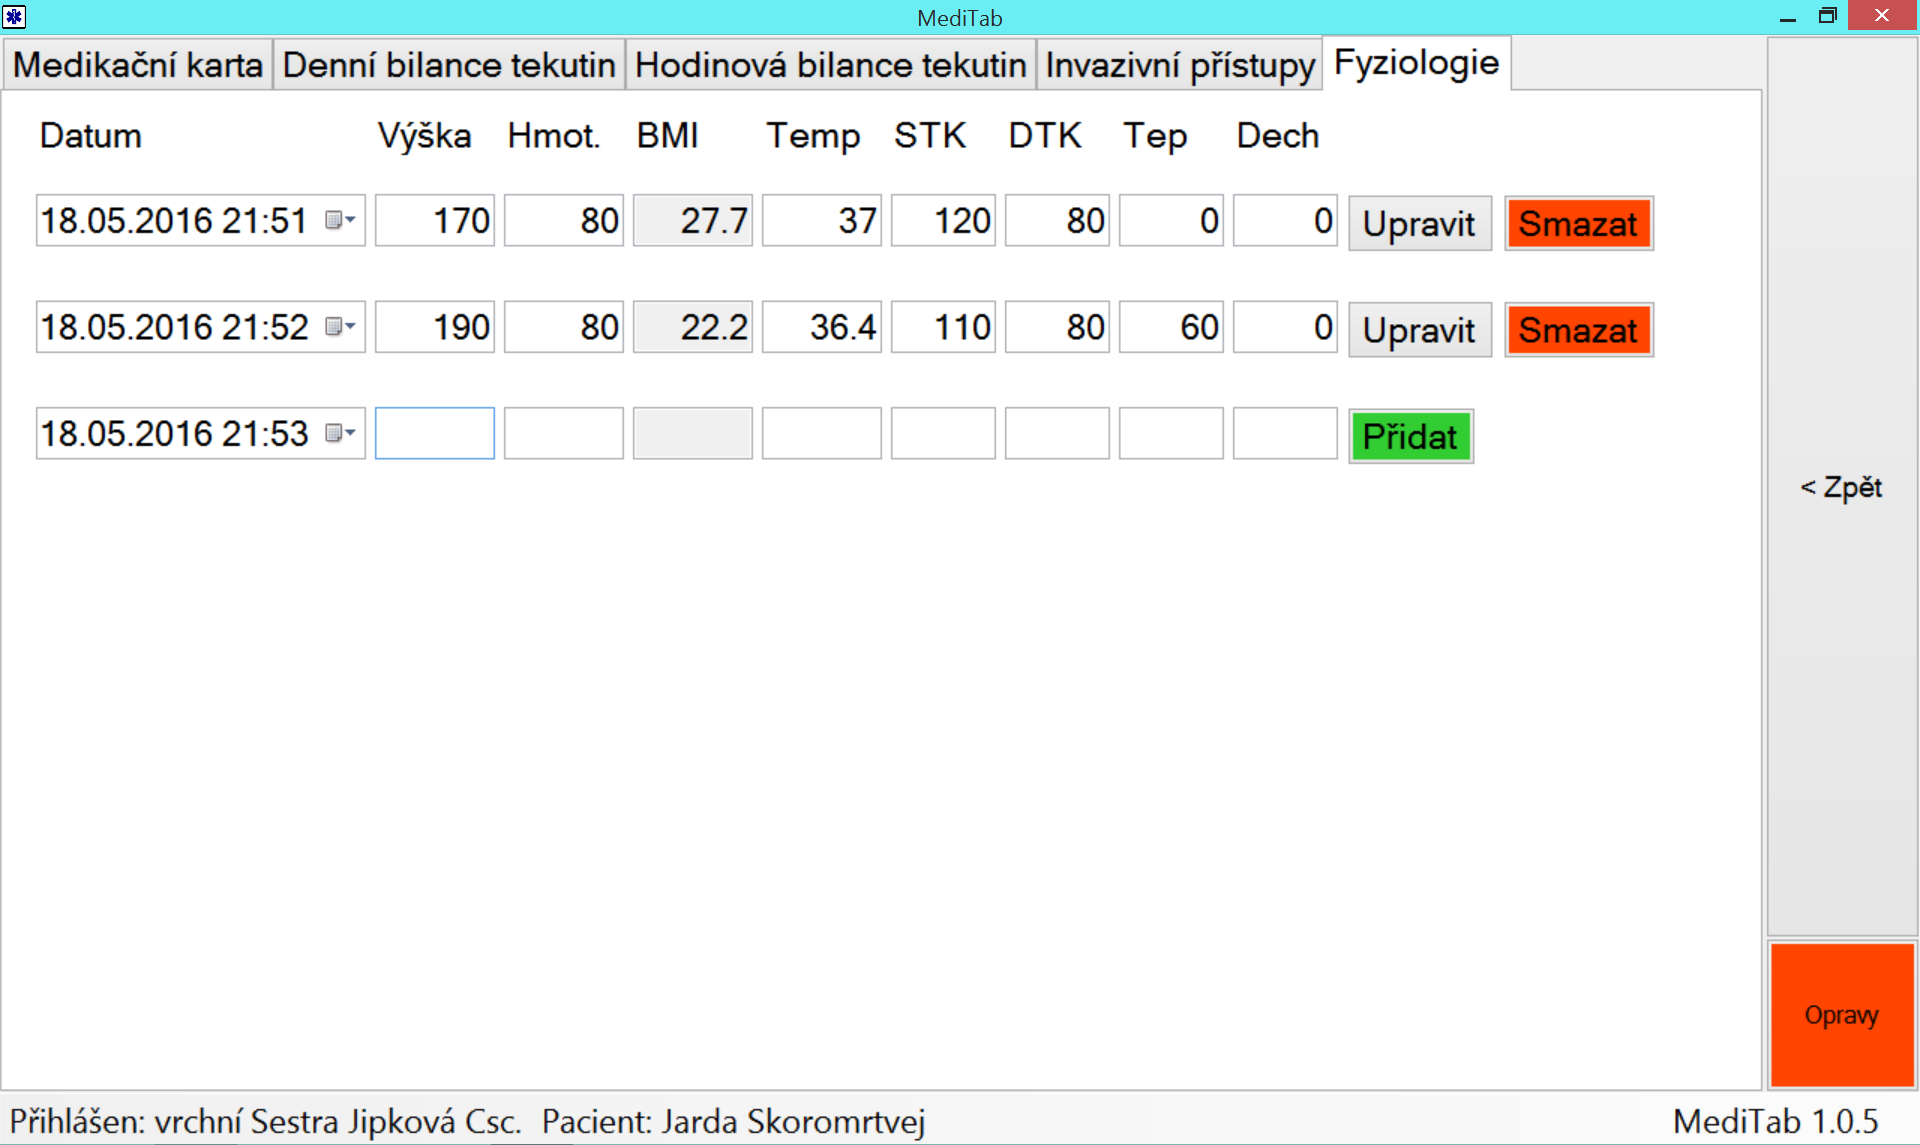
\includegraphics[width=1\textwidth]{img/meditab/fyziologie.eps}
	\caption{Fyziologie (MediTab)}
  \label{fig:fyziologie}
\end{figure}

Scrollování je opět vyřešeno pomocí MouseFilteru a TouchableFlowLayoutPanelu jako u invazivních přístupů (viz kapitola \ref{ch:pristup}).


\subsection{Opravy}

V dialogu oprav (na obrázku \ref{fig:opravy}) se zobrazují všechny akce provedené přihlášeným uživatelem na dané záložce. Každá akce je FlowLayoutPanel s časem provedení, popisem a Buttonem pro zrušení akce. Po zavření dialogu (Button \emph{Zavřít} vespod) se záložka aktualizuje.

\begin{figure}[H]
	\centering
	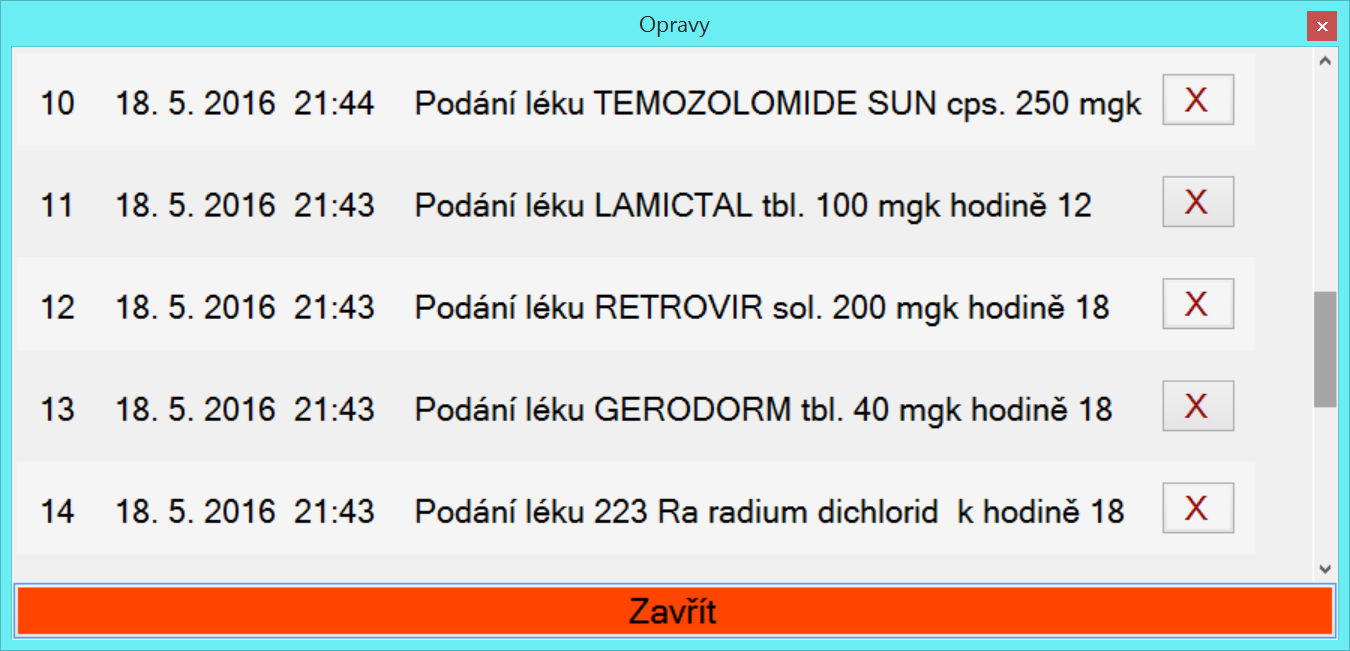
\includegraphics[width=0.8\textwidth]{img/meditab/opravy.eps}
	\caption{Opravy (MediTab)}
  \label{fig:opravy}
\end{figure}



\section{Dialogy}
\label{ch:dialogy}

Některé prvky poskytované knihovnou WinForms nejsou vhodné pro tablety. Například u MessageBoxu nelze změnit velikost písma. Proto jsem vytvořil vlastní MessageBox.

Také systémová klávesnice není optimální. Po kliknutí do textového pole se automaticky nezobrazí, ale musí se kliknout na malé tlačítko v liště. Pro numerickou klávesnici je nutné provést ještě o jeden klik víc. Při použití klávsnice často zakryla pole do kterého se zapisovalo a uživatel tak psal \emph{na slepo}. To v nemocnici není žádoucí a vedlo to k vytvoření vlastní klávesnice a numerické klávesnice.

\subsection{MessageBox}

Dialog MessageBoxu obsahuje TableLayoutPanel s dvěma řádky a jedním sloupcem. V prvním řádku je text zprávy, ve druhém tlačítka zarovnaná doprava. MessageBox se zobrazuje s jedním potvrzovacím Buttonem \emph{OK} (viz obrázek \ref{fig:messagebox_ok}), nebo s dvěma Buttony \emph{Ano/Ne} (viz obrázek \ref{fig:messagebox_yn}) a následně vrací DialogResult podle toho, na co uživatel klikl (DialogResult.Yes nebo DialogResult.No).

\subsection{Klávesnice}

Rozložení klávesnice odpovídá klasické klávesnici. Pro větší přehlednost neobsahuje veškeré speciální znaky, ale pouze ty, které jsou používány v nemocnici. V horní části je TextBox, ve kterém uživatel vidí co píše (viz orázek \ref{fig:keyboard}). Při zobrazení klávesnice může být TextBox již vyplněn textem z pole do kterého zapisujem. Vrací DialogResult.OK, pokud uživatel potvrdí zápis, nebo DialogResult.Cancel, pokud nepotvrdí.

\begin{figure}[H]
	\centering
	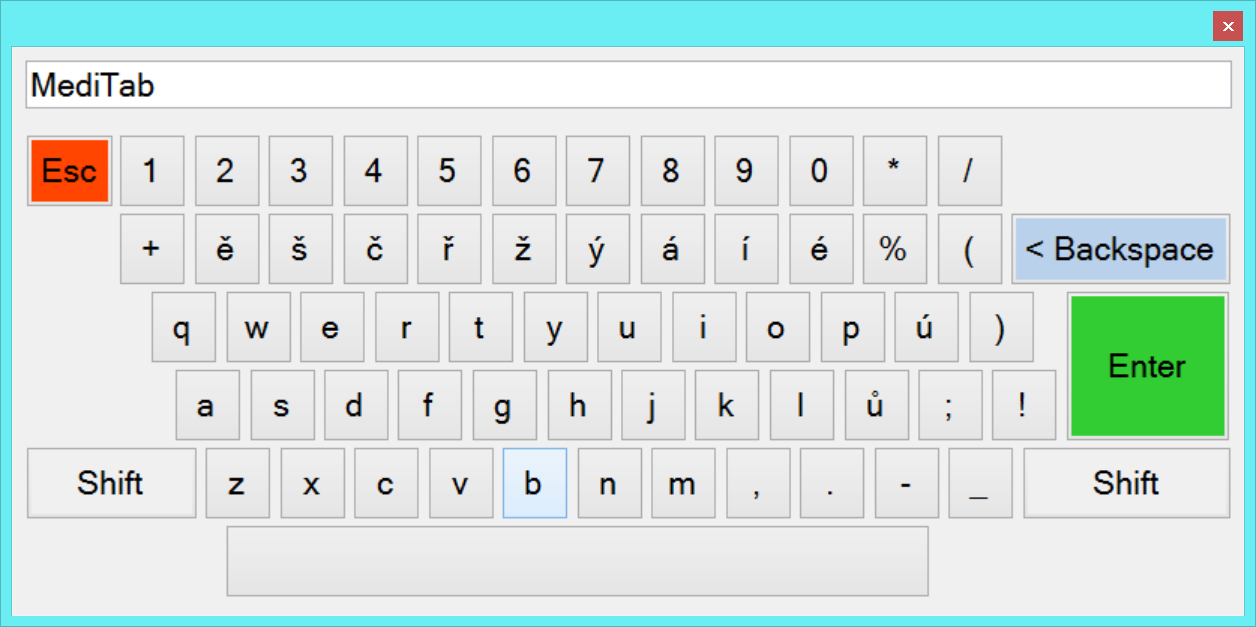
\includegraphics[width=0.8\textwidth]{img/meditab/keyboard.eps}
	\caption{Klávesnice (MediTab)}
  \label{fig:keyboard}
\end{figure}

\subsection{Numerická klávesnice}

Jednoduchá numerická klávesnice pouze s ciframi, desetinnou čárkou a potvrzovacími tlačítky (viz obrázek \ref{fig:keyboard_num}). Klávesnice má dva módy, s aktivní či neaktivní desetinnou čárkou. V horní části je TextBox stejně, jako je tomu u předešlé klávesnice. Vrací DialogResult.OK, pokud uživatel potvrdí zápis, nebo DialogResult.Cancel pokud nepotvrdí.

\begin{figure}[H]
	\centering
	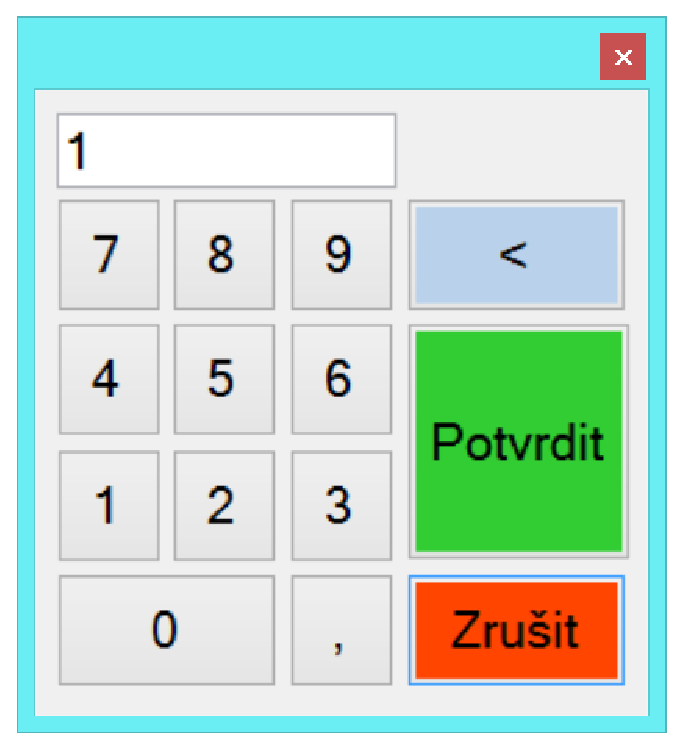
\includegraphics[width=0.3\textwidth]{img/meditab/keyboard_numeric.eps}
	\caption{Numerická klávesnice (MediTab)}
  \label{fig:keyboard_num}
\end{figure}